% ==========================================================================================
% PhD Thesis Template for Scuola Universitaria Superiore (IUSS) di Pavia 
% ==========================================================================================
% Feel free to keep in touch to let us know about any issues or suggestions for further improvements:
% Volkan Ozsarac <volkan.ozsarac@iusspavia.it> 
% Jimena Yanina Martin <jimena.martin@iusspavia.it>
%
% ==========================================================================================
% Editorial Notes vo 20/09/2021
% ==========================================================================================
% 1-) People from HYRIS curricula must comment lines 131-132 and uncomment lines 133-134 in IUSS_Thesis_Draft.cls, and vice a versa for people from ROSE curricula
% 2-) The font styles are not exactly identical with the template in word, therefore we have to improvise. Whatever we do there will be some differences between two templates which have to keep in mind.

% ==========================================================================================
% Remaining Issues in Template vo 20/09/2021
% ==========================================================================================
% 1-) Vertical spacing for all must be checked, and fixed if necessary.
% 2-) Font size for all must be checked, and fixed if necessary. If somebody finds a better font style
% solution we can adopt that (ebgaramond is not exactly the same as garamond in word).
% 3-) Format for the rest of the reference types must be added (for example, online sources) Currently we have the correct format for books, thesis, individual study, conference papers, article papers.
% 4-) Use of all the included packages must be specified to avoid confusion. Then we can remove unnecessary packages

\documentclass{Miscellaneous/IUSS_Thesis_Draft}
% ==========================================================================================
% Extra Packages
% ==========================================================================================
% These packages are not required in the template, can be used for other purposes.
% \usepackage{showframe} % To show frame
\usepackage{todonotes} % To add TODO notes
\usepackage{lipsum} % temporary package to fill document
\usepackage{blindtext} % temporary package to fill document

% ==========================================================================================
% Figure locations jmt 06/09/2021
% ==========================================================================================
% We can just set this to Figures, not sure if is very important though (VO)
% \graphicspath{Figures}

% ==========================================================================================
% Start of Document
% ==========================================================================================
\begin{document}

% ==========================================================================================
% Front Matter
% ==========================================================================================
\title{Insert Title of the UME PhD Thesis here} % Input the thesis name
\author{Name Surname} % Input the author
\date{February 2021}  % Input the delivery date
\nomenclature{$k$}{=Stiffness}
\nomenclature{$m$}{=Mass}
\nomenclature{$T$}{=Period of Vibration}
\nomenclature{$\pi$}{=Pi}
 % Retrieve the Nomenclature
\pagestyle{empty} % Remove the page number
\pagenumbering{roman} % Set page numbering to Roman for front matter
\advisor{} % First title does not have advisors
\maketitle % Make the first title page
\cleardoublepage % Insert an empty page
\advisor{Supervisors:\\First Advisor, Affiliation\\Second Advisor, Affiliation\\} % Second title page has advisors
\maketitle % Make the second title page
\cleardoublepage % Insert an empty page

\begin{abstract} % Abstract text goes here
This report contains guidelines for formatting a UME PhD Thesis using \LaTeX.
\end{abstract} % End the abstract

\begin{acknowledgements} % Acknowledgements text goes here
Acknowledegements can be provided here (though it is not compulsory to include them). 
\end{acknowledgements} % End the acknowledgements

\makeToC % Make table of contents
\makeLoF % Make list of figures
\makeLoT % Make list of tables
\makeLoS % Make list of symbols (Uses Nomentclature.tex insert symbol definitions there)
\cleardoublepage % Insert an empty page
\phantomsection	% Command is necessary for hyperref to jump to the correct page, in other words it puts a hyper marker on the page.
\pagestyle{fancy} % Not sure what does this do Jime? --> VO
\pagenumbering{arabic} % Set page numbering to arabic again

% ==========================================================================================
% Chapters
% ==========================================================================================
\chapter{Formatting Guidelines}
\section{Introduction}
Please read carefully the instructions presented herein for the format of a UME PhD thesis at the UME School, Pavia. This document has been written in the required format and so please study the document for any formatting requirements that are not explicitly stated in the text. Any formatting styles not described herein are left to the author’s discretion. 
\section{Setting up the Document}
The Page Setup option under the File toolbar in \LaTeX \space should be adapted as described in what follows. The margins for A4 size paper should be fixed thus: top 6cm, bottom 4.7cm, inside 4cm and outside 3.5cm. The \textit{Multiple Pages} option should be set to \textit{Mirror Margins}. On the \textit{Layout} tab of \textit{Page Setup}, the \textit{Section Start} should read \textit{Odd page} and the Headers and footers should have the options \textit{Different odd and even} and \textit{Different first page} both checked. The \textit{Header} and \textit{Footer} should be set at 4.8cm and 1.5cm from edge, respectively. To ensure that first page of each chapter and section is located on the right-hand side of the double-sided document, section breaks need to be inserted; the location of these breaks is denoted herein by: [Insert a Section Break (Odd Page)…..]. 
\section{Styles and Formatting}
\subsection{Fonts and Line Spacing}
A description of the fonts and line spacing used throughout the report is provided in Table \ref{tab:Styles}. Styles not included in Table \ref{tab:Styles} included bullet points which should be placed at 6pt after the paragraph and have the following format:
\begin{itemize}
    \item \todo{spacing should\\be adjusted}11pt Garamond with exactly 13pt spacing, 0pt before, 3pt after, and 0.63cm tab and 0.63cm hanging should be used in all bullet points,
    \item 11pt Garamond with exactly 13pt spacing, 0pt before, 3pt after, and 0.63cm tab and 0.63cm hanging should be used in all bullet points.
\end{itemize}
The last bullet point should have 0pt before, 13pt after spacing.
% Table generated by Excel2LaTeX from sheet 'Sheet1'

\begin{table}[hbtp]
  \centering
  \small
  \todo[inline]{Vertical spacing requirements for all in this table needs to be checked or addressed}
  \caption{Description of the styles used in the UME PhD Thesis}
    \begin{tabularx}{\textwidth}{|p{2.5cm}|L|}
    \hline 
    \parnoteclear % tabularx will otherwise add each note thrice
    \textbf{Heading 1} & \textbf{Heading 2} \\
    \hline 
    Acknowledgements Title\parnote{Table Footnote 1}  & 14pt Garamond, ALL CAPS, bold, 60pt before, 18pt after, centred.\\
    \hline
    Acknowledgements text\parnote{Table Footnote 2} & 11pt Garamond, 0pt before, 13pt after, exactly 13pt line spacing.\\
    \hline
    Table of Contents Title & 14pt Garamond, ALL CAPS, bold, 60pt before, 18pt after, centred.\\
    \hline
    Table of Contents & Insert Table using Insert, Reference, Index and Tables, show page numbers, right-align page numbers, dotted tab leader, Garamond 10pt, 6pt before, 6pt after, single spacing \\
    \hline
    List of Tables / Figures / Symbols Title & 14pt Garamond, ALL CAPS, bold, 60pt before, 18pt after, centred. \\
    \hline
    List of Tables / Figures & Show and right-align page numbers, tab leader dotted, Garamond 10pt, 6pt before, 6pt after, single spacing, indentation right 0.25cm, hanging 1.8cm \\
    \hline
    List of Symbols & Alphabetical list of Roman letters then Greek Letters, Garamond 10pt. \\
    \hline
    Header & 9pt Garamond, bold, Odd pages: Name of Thesis, centred, page number right aligned, Even pages: Name of Author, centred, page number left aligned \\
    \hline
    Heading 1 & 14pt Garamond, ALL CAPS, bold, 60pt before, 18pt after, left-aligned \\
    \hline
    Heading 2 & 11pt Garamond, Small Caps, bold, 6pt before, 6pt after,           0.63cm tab \\
    \hline
    Heading 3 & 11pt Garamond, 1st letter Caps, bold, 6pt before, 6pt after, 1 cm tab \\
    \hline
    Heading 4 & 11pt Garamond, 1st letter Caps, Italic, bold. \\
    \hline
    Body Text & 11pt Garamond, 0pt before, 13pt after, exactly 13pt spacing, justified \\
    \hline
    Figure caption & Below figure, 9pt Garamond, bold, 6pt before, 6pt after, single spacing, justified when > 1 sentence, otherwise centred. \\
    \hline
    Table Text & Header: 10pt Garamond, bold, 3pt before, 3pt after, single spacing, Row: 10pt Garamond, 2pt before, 2pt after, single spacing, \\
    \hline
    Table caption & Above table, 9pt Garamond, bold, 6pt before, 6pt after, single spacing, left-aligned \& justified, or centred (see Section 1.3.4) \\
    \hline
    References (list) & 10pt Garamond, 0pt before, 13pt after, exactly 13pt spacing, hanging 0.75cm \\
    \hline
    Reference Title & 14pt Garamond, ALL CAPS, bold, 60pt before, 18pt after, centred \\
    \hline
    \end{tabularx}
    \label{tab:Styles}
    \raggedright\parnotes
\end{table}%

Numbered lists should be placed at 6pt after the paragraph and be formatted with Roman numerals in the following way:
\begin{enumerate}
    \item \todo{spacing should\\be adjusted}11pt Garamond with exactly 13pt spacing, 0pt before, 3pt after, and 0.63cm tab and 0.63cm hanging should be used in all numbered lists,
    \item The last numbered list should have spacing 0pt before and 13pt after.
\end{enumerate}

Footnotes should be numbered sequentially in superscript lowercase Roman letters\footnote{Footnotes should be typeset in 9pt Garamond at the bottom of the page.}.

\subsection{The Body Text}
The language of the main text should be set to English (U.K.). Abbreviations are allowed but should be spelt out in full when first used. Integers of ten and below are to be spelt out. Foreign language phrases should be italicised (e.g., Latin, French).

\subsection{Header and Page Numbering}
The header should vary for the first, odd and even pages: there should be no header on the first page of each section/chapter, on odd pages the title of the PhD thesis should be inserted (though it should not run onto a second line and may thus need to be shortened) whilst the name of the author(s) should be placed on the header of even pages.  The format of the text in the header is described in Table \ref{tab:Styles}. Page numbers (9pt Garamond, bold) are included in the headers and should be flush outside. The preliminary pages of the thesis from the Abstract to the last page of the Table of Figures should be numbered using Roman numerals (i.e. i, ii, iii).  The page numbers should restart using Arabic numbers (i.e. 1, 2, 3) on the first page of Chapter 1 and should continue until the last page of the report/thesis.

\subsection{Equations, Figures and Tables}
Equations should be centred within the text width, whilst equation numbers should be placed in parentheses and set flush with the right margin, as illustrated in Equation \eqref{eqn:Period}:

\begin{equation}
    \label{eqn:Period}
    T=2\pi\sqrt{\frac{m}{k}}
\end{equation}

In equations, the text, variables and functions should be in \textit{Italic}, whilst numbers and functions should not (see Figure \ref{fig:size_of_symbols} for a description of styles sizes and Figure \ref{fig:style_of_symbols} for a description of the style fonts to be used in equations). The sequence of signs in equations should generally be \{[(  )]\}, with due account taken of the special meaning of certain types of brackets. Standard letters such as x are to appear as x (italicised) in the text if they are used as mathematical symbols.\par
Figures should be included in the report as illustrated in Figure \ref{fig:size_of_symbols}; there should be 3pt space before and 6pt space after each figure. A caption should be inserted ideally using the \textit{Insert – Reference – Caption} option in Word using the format described in Table \ref{tab:Styles}. In \LaTeX \space just use \slash{caption\{\}}. The captions of figures should be centred if one line only, otherwise they should be justified; the second line of the caption should begin beneath the text of the first line. 

\begin{figure}[hbt!]
    \centering
    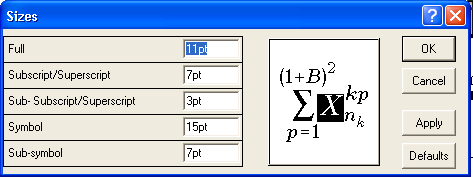
\includegraphics[width=0.7\textwidth]{Equation_Font.png}
    \caption{Screenshot of the sizes of symbols to be used in equations in a UME PhD Thesis taken from Microsoft Equaton 3.0}
    \label{fig:size_of_symbols}
\end{figure}

\begin{figure}[hbt!]
    \centering
    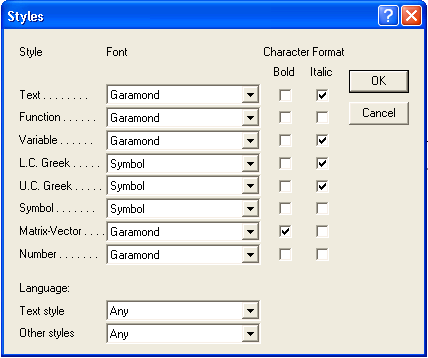
\includegraphics[width=0.7\textwidth]{Equation_Style.png}
    \caption{Screenshot of the styles to be used in equations in a UME PhD Thesis taken from Microsoft Equation 3.0}
    \label{fig:style_of_symbols}
\end{figure}

Tables should have either the format shown in Table \ref{tab:empty_narrow} or Table \ref{tab:empty_wide}; the former format is recommended for simple tables with limited rows and columns. The captions of tables should be left-aligned and justified when the table is wide (as in Table \ref{tab:Styles} and Table \ref{tab:empty_wide}) and if the caption exceeds one sentence, the second line should begin beneath the caption text of the first line. If the table has only a few columns and is narrow (as in Table \ref{tab:empty_narrow}) then the caption should be centred within the width of the table. 

\begin{table}[hbtp]
  \centering
  \captionsetup{width=0.6\textwidth}
  \caption{Table captions for narrow tables should be centred within the width of the table like this}
    \begin{tabularx}{0.6\textwidth}{L L L}
    \hline
     & & \\
    \hline
     & & \\
     & & \\
     & & \\
     \hline
    \end{tabularx}
  \label{tab:empty_narrow}
\end{table}

\begin{table}[hbtp]
  \centering
  \caption{Table captions that are longer than one sentence should be justified and the second line should begin directly below the start of the text in the first line} 
    \begin{tabularx}{\textwidth}{|L|L|L|L|L|}
    \hline
    \parnoteclear % tabularx will otherwise add each note thrice
     & & & & \parnote{Table Footnote 1}\\
    \hline
     & & & & \\
     \hline
     & & & & \\
     \hline
     & & & & \\
     \hline
     & & & & \\
     \hline
    \end{tabularx}
    \raggedright\parnotes
  \label{tab:empty_wide}
\end{table}

\subsubsection{Example of a Fourth Level Heading.} 
This is an example of a fourth level heading. These headings should not be included in the Table of Contents. There should be two spaces after the letter (a), (b) etc. and two spaces after the title (Bold, Italic, Garamond 11pt).

\subsection{Graphs, Pictures and Photos}
As a general rule, PhD theses are to be printed in Black \& White, hence, authors should make an effort to produce plots in which colour printing is not a prerequisite to make these easily understood and interpreted.\par
Therefore, and as an example, the employment of different line styles (varying the dash type, thickness, using point markers etc.) is preferred to the use of different colours. It is noted that not all software packages manage to produce quality plots when dashed lines are used, hence authors are invited to first test out some plots samples before embarking on mass production of graphs.
\subsection{References}
All references should be cited in the text by name and year and may take one of the following forms: “…as shown by Miller [1967], the…” or “…has often been demonstrated [Smith and Jones, 2002a, 2002b; Brown et al., 2003] that…” The reference list should be placed at the end of the thesis, but before any appendices, and must be in alphabetical order by first authors’ surnames and presented in the style shown in the examples in the reference section of these guidelines. Lets place some citations here: \\
two citations at a time: \citep{abrahamson1997empirical, pinto2004seismic} \\
citation with two authors: \cite{abrahamson2005opinion} \\
citation with more than two authors: \cite{pinto2004seismic}  \\
citation with single author: \cite{abrams1992strength} \\
citation with single author: \cite{crowley2005investigative} \\
citation with single author: \cite{icc:2003}

\subsection{Appendices}
Any appendices included in the document should be numbered alphabetically and placed at the end of the thesis after the references (see example at the end of this document). \par
[Insert a Section Break (Odd Page) at the end of each Chapter]


\chapter{A New Chapter}
\section{A New Section}
\blindtext
\subsection{A New Subsection}
\blindtext
\subsubsection{Example of a Fourth Level Heading.} 
\blindtext
\subsubsection{Example of another Fourth Level Heading.} 
\blindtext

\subsection{Another Subsection}
\lipsum
\section{A New Section}
\lipsum


% ==========================================================================================
% References
% ==========================================================================================
\makebib
\todo[inline]{Other reference types need to be checked and fixed if necessary}
% ==========================================================================================
% Appendices
% ==========================================================================================
\clearpage
\phantomsection
\addcontentsline{toc}{chapter}{Appendix A. Type Title Here}
\part*{Appendix A. Type Title Here}
\thispagestyle{empty} % I added this because these page numbers are not shown in word template
Some appendix stuff are inserted here
\renewcommand{\thetable}{A.\arabic{table}}
\begin{table}[hbtp]
  \centering
  \captionsetup{width=0.7\textwidth}
  \caption{An appendix table}
    \begin{tabularx}{0.7\textwidth}{L L L}
    \hline
    First column & Second Column & Third column\\
    \hline
    First row & First row & First row\\
    Second row & Second Row & Second Row\\
    \hline
    \end{tabularx}
  \label{tab:appendix_table_1}
\end{table}
\clearpage
\phantomsection
\addcontentsline{toc}{chapter}{Appendix B. Type Title Here}
\part*{Appendix B. Type Title Here}
\thispagestyle{empty} % I added this because these page numbers are not shown in word template
Some other appendix stuff are inserted here

% ==========================================================================================
% End of Document
% ==========================================================================================
\end{document}
